Im folgenden Kapitel sollen die wichtigsten physikalischen Grundlagen für das
Verständnis der in dieser Arbeit behandelten Thematik erklärt werden. Dabei
werden die Kenntnisse über den Aufbau des Atoms, die quantisierten Lösungen der
Schrödinger- bzw. Diracgleichung, die dabei auftretenden Drehimpulskopplungen
und die daraus resultierenden Energieaufspaltungen der Atome als vorhanden
vorausgesetzt. Diesbezüglich sei auf einschlägige Lehrbücher wie
\cite{demtroeder:ex3}, \cite{demtroeder:laserspektroskopie} und \cite{saleh:grundlagen_der_photonik}
verwiesen. In Kapitel \ref{sec:licht-atom-wechselwirkung} soll die
Wechselwirkung von Licht und Atom behandelt werden. Darauf aufbauend soll
in Kapitel \ref{sec:ris} die Resonanz-Ionisations-Spektroskopie,
kurz RIS, in Bezug auf die Resonanz-Ionisation von Uran-Isotopen erklärt
werden. Kapitel \ref{sec:diodenlaser} soll das Funktionsprinzip von
Halbleiterlasern und deren Rolle in diesem Projekt wiedergeben.

\section{Licht-Atom-Wechselwirkung}\label{sec:licht-atom-wechselwirkung}
Essenziell wichtig für die Resonanz-Ionisation ist das Verständnis der atomaren
Wechselwirkung mit einem elektromagnetischen Feld. Im Folgenden soll insbesondere auf die
atomaren Übergänge und deren Linienprofil eingegangen werden, da dies bei der
Atom-Spektroskopie eine wichtige Rolle spielt. Der größte Teil der dieses
Theorie-Abschnitts basiert im Wesentlichen auf den o.g. Lehrbüchern.

% $$P_{ik}=\frac{2\pi}{\hbar^2}\lvert\langle\psi_k^0\rvert\hat{\mathcal{H}}'\lvert\psi_i^0\rangle\rvert^2\delta(E_k^0-E_i^0+\hbar\omega)$$
% $$W_{ki}=\frac{\pi e^2}{3\varepsilon_0\hbar^2}\lvert\langle\psi_k\rvert\vec{r}\lvert\psi_i\rangle\rvert^2\cdot\omega_{\nu}$$
% $$B_{ki}=\frac{2}{3}\frac{\pi^2e^2}{\varepsilon_0\hbar^2}\lvert\langle\psi_k\rvert\vec{r}\lvert\psi_i\rangle\rvert^2$$
% $$\vec{M}_{ik}=e\langle\psi_i\rvert\vec{r}\lvert\psi_k\rangle$$
% $$\langle p\rangle = e\langle r\rangle = e\langle\psi_i\rvert
% r\lvert\psi_i\rangle$$
% $$\lvert\psi_k\rangle$$
% $$\bar p ^2 \rightarrow \frac{1}{2}(\lvert M_{ik}\rvert+\lvert M_{ik}\rvert)^2 =
% 2\lvert M_{ik}\rvert^2$$


\subsection{Übergangsraten}\label{subsec:uebergangsraten}
Befindet sich ein Atom in einem elektromagnetischen Feld können Absorptions- und
Emissions-Prozesse beobachtet werden. Im ersten Fall absorbiert das Atom ein
Photon einer bestimmten Mode mit der Energie $\hbar\omega_L$ aus dem elektromagnetischen Feld.
Dabei wird das Atom von einem Zustand in einen entsprechend der Photonenenergie
energetisch höher gelegenen Zustand überführt:
\begin{equation}\label{eq:uebergang}
	E_f-E_i=\hbar\omega_L
\end{equation}
Dabei ist zu beachten, dass gebundene Zustände immer quantisiert sind, also
nicht kontinuierlich im Energiespektrum verteilt sind. Analog kann ein Atom ein
Photon in das elektromagnetische Feld emittieren\footnote{Die Emission ist
auch ohne Feld möglich. Dieser Fall wird \textit{spontane Emission} genannt}.
Die Zustandsänderung des Atoms folgt dann entsprechend von einem Zustand in ein energetisch niedriger gelegenen Zustand.\par

\subsubsection{Fermis goldene Regel}\label{subsubsec:fermis_goldene_regel}
Grundlegend beschreibt \textit{Fermis goldene Regel} die
Übergangsrate von einem Zustand $\Psi_i$ (i: \textit{initial}) in einen
beliebigen Zustand $\Psi_f$ (f: \textit{final}). Diese kann halbklassisch
störungstheoretisch hergeleitet werden.  Dabei betrachtet man das externe elektromagnetische Feld als Störung
zusätzlich zum zeitunabhängigen Hamilton-Operator $\OPH_0$:
\begin{equation}\label{eq:hamilton}
	\OPH(t)=\OPH_0+\OPH'(t)
\end{equation}
mit dem Wechselwirkungsoperator
\begin{equation}\label{eq:ww}
	\begin{split}
		\OPH'(t) &= -E_0\vec{\epsilon}\cdot\OPv{d}\cos{(\vk\cdot\vr-\omega_L t)}\\
		&=
		-\OPH'\left(\mathrm{e}^{\mathrm{i}(\vk\cdot\vr-\omega_L
		t)}+\mathrm{e}^{-\mathrm{i}(\vk\cdot\vr-\omega_L t)}\right)\\
		&\text{mit}\quad
		\OPH'=\frac{1}{2}E_0\vec{\epsilon}\cdot\OPv{d}\,.
	\end{split}
\end{equation}
Hierbei ist $E_0$ die Amplitude und $\vec{\epsilon}$ der
Polarisierungsvektor des elektromagnetischen Feldes. $\OPv{d} = e\OPv{r}$ ist
der Dipoloperator. Zusätzlich kann man die Annahme machen, dass das Atom in Relation zur
Wellenlänge des Lichts sehr klein ist und es somit am Ort
des Atoms nur verschwindend geringe örtliche Änderungen der Amplitude des
elektromagnetischen Feldes erfährt ($\vk\cdot\vr\ll 1$, Atom am Ort $\vr=0$). Diese Näherung nennt man
\textit{Dipolnäherung}. Dadurch folgt für die Entwicklung des
Ortsteils der Exponentialfunktionen in erster Ordnung
$\mathrm{e}^{\pm\mathrm{i}\vk\cdot\vr}\approx1$. Nun setzt man mit der zeitabhängigen Schrödingergleichung an und entwickelt $\Psi(t)$ in die stationären Eigenzustände $\Psi_n$ des Atoms:
\begin{equation}\label{eq:sgl_stoerung_01}
	\mathrm{i}\hbar\pfrac{}{t}\ket{\Psi(t)}=\OPH(t)\ket{\Psi(t)}\,,
	\quad
	\ket{\Psi(t)}=\sum\limits_n{c_n(t)\mathrm{e}^{-\frac{\mathrm{i}}{\hbar} E_n
	t}\ket{\Psi_n}}
\end{equation}
Führt man die Zeitableitung aus und projiziert beide Seiten der Gleichung auf
einen beliebigen Zustand $\Psi_f$, findet man
\begin{equation}\label{eq:sgl_stoerung_02}
	\dot
	c_f(t)=-\frac{\mathrm{i}}{\hbar}\sum\limits_n{c_n(t)\mathrm{e}^{-\mathrm{i}\omega_{nf}t}\bra{\Psi_f}\OPH'(t)\ket{\Psi_n}}
	\quad\text{mit}\quad
	\omega_{nf}=\frac{E_n-E_f}{\hbar}\,.
\end{equation}
Nimmt man nun an, dass die Störung klein ist, das Atom also vornehmlich im
Ausgangs-Zustand $\Psi_i$ bleibt ($c_i(0)=1$, $c_i(t)\approx 1$, $c_{n\neq
i}\approx0$), verkürzt sich die Summe in Gl. \eqref{eq:sgl_stoerung_02}
auf einen Summanden mit $n=i\neq f$. $c_f(t)$ folgt aus zeitlicher Integration von $\dot c_f(t)$ mit
Gl. \eqref{eq:ww}:
\begin{equation}\label{eq:koeff_cf}
	\begin{split}
		c_f(t) &= \int_0^t{\dot c_f(t')\dd t'}\\
		&=
		-\frac{\mathrm{i}}{\hbar}\bra{\Psi_f}\OPH'\ket{\Psi_i}\left[\frac{\mathrm{e}^{\mathrm{i}(\omega_{fi}-\omega_L)t}-1}{\mathrm{i}(\omega_{fi}-\omega_L)}+\frac{\mathrm{e}^{\mathrm{i}(\omega_{fi}+\omega_L)t}-1}{\mathrm{i}(\omega_{fi}+\omega_L)}\right]\\
		&\text{mit}\quad
		\omega_{fi}=-\omega_{if}
	\end{split}
\end{equation}
Zu beachten ist hierbei, dass im Falle der Absorption der Nenner des zweiten
Bruchs in Gl. \eqref{eq:koeff_cf} im nahresonenten Fall
($\omega_{fi}\approx\omega_L$) in der Größenordnung $2\omega_{fi}\approx
10^{15}\,\text{s}^{-1}$ (bei optischen Übergängen) liegt. Somit wird der
zweite Bruch verschwindend gering gegenüber dem ersten und kann vernachlässigt
werden. Im Falle der Emission betrachtet man Übergänge vom energetisch höheren
Niveau zum energetisch niedrigeren Niveau. Dabei gilt
($\omega_{if}\approx\omega_L$), wodurch der erste Bruch vernachlässigt werden
kann. Diese Näherung wird auch \textit{Rotating-Wave-Approximation} (kurz RWA)
genannt. Im Folgenden wird allerdings exemplarisch die Absorption betrachtet.
Für die Übergangswahrscheinlichkeit ergibt sich
\begin{equation}\label{eq:uebergangs_wkt}
	\begin{split}
		P_{i\to f}(t,\Delta\omega) &= \abs{c_f(t)}^2\\
		& =
		\frac{1}{\hbar^2}\abs{\bra{\Psi_f}\OPH'\ket{\Psi_i}}^2\cdot\frac{\sin^2{\left(\frac{\Delta\omega}{2}t\right)}}{\left(\frac{\Delta\omega}{2}\right)^2}\\
		&\text{mit}\quad
		\Delta\omega=\omega_L-\omega_{fi}\,.
	\end{split}
\end{equation}
Für die totale Übergangswahrscheinlichkeit gilt dann mit Gl.
\eqref{eq:uebergangs_wkt}
\begin{equation}\label{eq:uebergangs_wkt_total}
	\begin{split}
		P_{i\to f}(t)
		&= \int{P_{i\to f}(t,\Delta\omega)\rho(E_f)}\dd E_f\\
		&\approx \rho(E_f)\int{P_{i\to f}(t,\Delta\omega)}\dd E_f\\
		&= \hbar\rho(E_f)\int_{-\infty}^{\infty}{P_{i\to
		f}(t,\Delta\omega)}\dd(\Delta\omega)\\
		&= \frac{2\pi t}{\hbar}\rho(E_f)\abs{\bra{\Psi_f}\OPH'\ket{\Psi_i}}^2\,.
	\end{split}
\end{equation}
Hierbei wurde die Energieniveaudichte $\rho(E_f)=\fracd{n}{E_f}$ eingeführt. Sie
beschreibt die Verteilung der Energieniveaus der Endzustände $E_f$. Mit anderen
Worten: Man nimmt nicht mehr ein diskretes Endniveau an, sondern eine Kontinuum
von Endzuständen. Mit der Annahme, dass sich $\rho(E_f)$ gegenüber $P_{i\to
f}(t,\Delta\omega)$ nur langsam ändert, kann $\rho(E_f)$ in Gl. \eqref{eq:uebergangs_wkt_total} als hinreichend konstant angenommen und aus dem Integral gezogen werden. Weiterhin wurde die Substitution $\dd E_f=\hbar\dd(\Delta\omega)$ vorgenommen. Für die
totale Übergangsrate folgt dann mit Gl. \eqref{eq:uebergangs_wkt_total}
für genügend große Zeiten ($t\to\infty\stackrel{\wedge}{=}
t\gg\frac{1}{\omega_{fi}}$) Fermis
goldene Regel:
\begin{equation}\label{eq:uebergangs_rate_total}
	\boxed{
		\begin{split}
			\Gamma_{i\to f}
			&= \lim_{t\to\infty}{\left(\fracd{}{t}{P_{i\to f}(t)}\right)}\\
			&= \frac{2\pi}{\hbar}\rho(E_f)\abs{\bra{\Psi_f}\OPH'\ket{\Psi_i}}^2
		\end{split}
	}
\end{equation}
$\bra{\Psi_f}\OPH'\ket{\Psi_i} =
\frac{1}{2}E_0\vec{\epsilon}\cdot e\bra{\Psi_f}\OPv{r}\ket{\Psi_i}$ enthält
das sog. \textit{Dipolmatrixelement} $e\bra{\Psi_f}\OPv{r}\ket{\Psi_i}$ für die Zustände
$\Psi_i$ und $\Psi_f$. Es gibt an, ob ein Übergang im Rahmen der Dipolnäherung
erlaubt oder verboten ist. Dazu sei auf Kapitel \ref{subsec:auswahlregeln}
verwiesen. Man erkennt zum einen, dass die Übergangsrate proportional zum
Betragsquadrat des Matrixelements ist und es zum anderen logischerweise keinen
Übergang zu nicht existenten Niveaus gibt ($\rho(E_f)=0$). 

\subsubsection{Einsteinkoeffizienten}\label{subsubsec:einsteinkoeffizienten}
Bisher wurden Absorption und Emission nur allgemein behandelt. Bei der Emission
muss man allerdings zwischen der \textit{induzierten} und der \textit{spontanen
Emission} unterscheiden. Die induzierte Emission findet nur mit vorhandenem
elektromagnetischen Feld statt. Es wird ein Photon der entsprechenden Mode aus
dem elektromagnetischen Feld benutzt, um eine Emission zu induzieren und ein
weiteres Photon in das Feld zu emittieren. Bei der spontanen Emission hingegen
fällt das Atom spontan in einen energetisch niedrigeren Zustand und ein
Photon der entsprechenden Mode wird emittiert (auch ohne Feld). In einem
elektromagnetischen Feld mit spektraler Energiedichte $w(\nu)=n(\nu)h\nu$, bei
der $n(\nu)=\pfrac{n}{\nu}$ die spektrale Photonendichte (also Photonendichte
pro Mode) ist, sind im stationären Gleichgewicht die Besetzungszahlen $N_i$ des
höheren Niveaus und $N_k$ des niedrigeren Niveaus zeitlich konstant. In der Ratengleichung
\begin{equation}\label{eq:raten_gleichung}
	A_{ik}N_i+B_{ik}w(\nu)N_i=B_{ki}w(\nu)N_k
\end{equation}
sind hierfür Emissionsraten und Absorptionsraten gleichgesetzt.
Die beiden Größen

\begin{subequations}\label{eq:einsteinkoeff_wkten}
	\begin{equation}\label{eq:einsteinkoeff_wkten_ik}
		W_{ki}=B_{ki}w(\nu)
	\end{equation}
	\begin{equation}\label{eq:einsteinkoeff_wkten_ki}
		W_{ik}=B_{ik}w(\nu)
	\end{equation}	
\end{subequations}
geben die Wahrscheinlichkeiten für die Absorption (a) und die induzierte
Emission (b) an, wobei $B_{ki}$ bzw. $B_{ki}$ die jeweiligen sog.
\textit{Einsteinkoeffizienten} sind. $A_{ik}$ ist der Einsteinkoeffizient für
die spontane Emission. Zeichnung \ref{fig:einstein_koeffizienten}
veranschaulicht dies.
\begin{figure}[h]
	\centering
	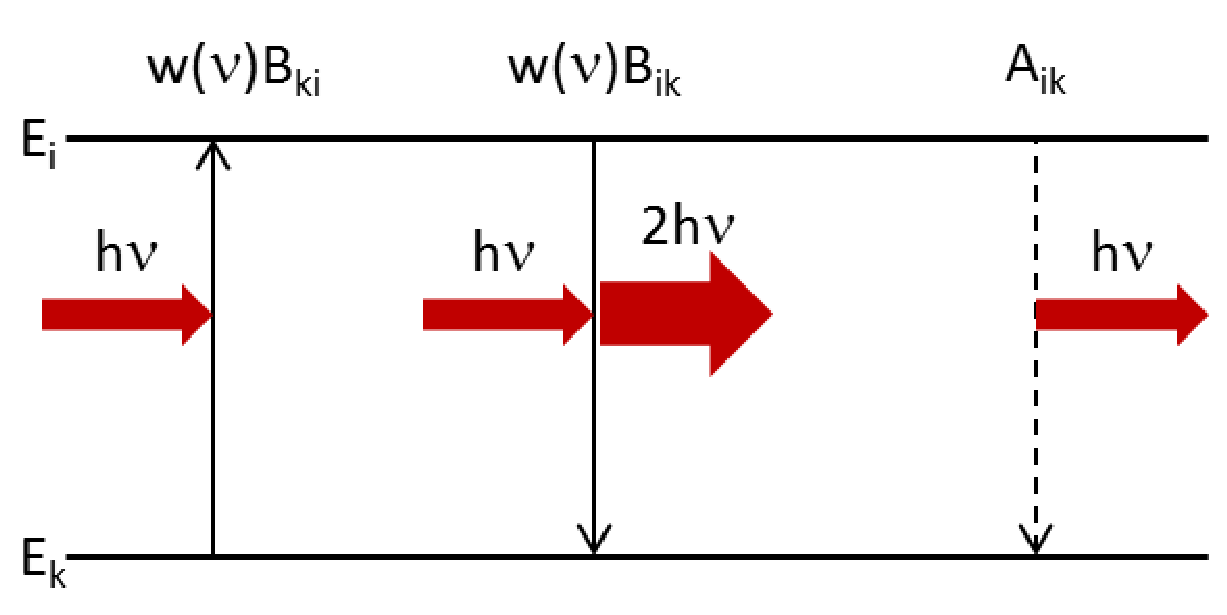
\includegraphics[width=10cm]{gfx/einstein_koeffizienten}
	\caption{zwei Energieniveaus eines Atoms mit Absorption,
	induzierte Emission und spontane Emission (von links nach
	rechts)}\label{fig:einstein_koeffizienten}
\end{figure}
Im thermischen Gleichgewicht sind die Besetzungszahlen
boltzmann-verteilt \cite{demtroeder:ex3}:
\begin{equation}\label{eq:boltzmann_verteilung}
	\begin{split}
		\frac{N_i}{N_k}&=\frac{g_i}{g_k}\mathrm{e}^{-\frac{(E_i-E_k)}{kT}}\\[0.2cm]
		&=\frac{g_i}{g_k}\mathrm{e}^{-\frac{h\nu}{kT}}\,.
	\end{split}	
\end{equation}
$g_i$ und $g_k$ sind die Entartungsgrade ($2J+1$) der jeweiligen Niveaus und
sind damit eine statistische Gewichtung der Niveaus.
Kombiniert man \eqref{eq:raten_gleichung} und \eqref{eq:boltzmann_verteilung}
und löst nach $w(\nu)$ auf, findet man
\begin{equation}\label{eq:spektrale_energiedichte_1}
	w(\nu)=\frac{\nicefrac{A_{ik}}{B_{ik}}}{\left(\nicefrac{g_i}{g_k}\right)\left(\nicefrac{B_{ik}}{B_{ki}}\right)\left(\mathrm{e}^\frac{h\nu}{kT}-1\right)}\,.
\end{equation}
Führt man einen Koeffizientenvergleicht mit der spektralen
Energiedichte eines thermischen Strahlungsfeldes \cite{demtroeder:ex3}
\begin{equation}\label{eq:spektrale_energiedichte_2}
	w(\nu)=\frac{8\pi h\nu^3}{c^3}\frac{1}{\mathrm{e}^\frac{h\nu}{kT}-1}
\end{equation}
durch, findet man folgende Beziehungen der Einsteinkoeffizienten:
\begin{subequations}\label{eq:einsteinkoeff_relationen}
	\begin{equation}\label{eq:einsteinkoeff_relationen_1}
		B_{ik}=\frac{g_k}{g_i}B_{ki}
	\end{equation}
	\begin{equation}\label{eq:einsteinkoeff_relationen_2}
		A_{ik}=\frac{8\pi h\nu^3}{c^3}B_{ik}\,.
	\end{equation}
\end{subequations}
**blabla01**
\par
Im Folgenden sollen die Einsteinkoeffizienten berechnet werden.
Zur Berechnung des Koeffizienten der spontanen Emissionswahrscheinlichkeit
betrachtet man das Atom als Hertzschen Dipol, der radial isotrop abstrahlt. Die
zeitlich mittlere abgestrahlte Leistung von $N_i$ Atomen
\cite{demtroeder:ex3} ist
\begin{equation}\label{eq:abgestrahlte_leistung_01}
	\mean{P}_t = \frac{1}{3}N_i\frac{\omega_{ik}^4}{\pi\epsilon_0
	c^3}\abs{\OPv{d}_{ik}}^2
\end{equation}
mit dem bereits erwähnte Dipolmatrixelement
$\OPv{d}_{ik}=e\bra{\Psi_i}\OPv{r}\ket{\Psi_k}$. Definiert man den
Einsteinkoeffizienten der spontanen Emission $A_{ik}$ als Wahrscheinlichkeit pro
Sekunde, dass ein Atom spontan von $\ket{\Psi_i}$ in $\ket{\Psi_k}$ übergeht,
ist Gl. \eqref{eq:abgestrahlte_leistung_01} identisch mit
\begin{equation}\label{eq:abgestrahlte_leistung_02}
	\mean{P}_t=N_iA_{ik}h\nu_{ik}\,.
\end{equation}
Daraus folgt
\begin{equation}\label{eq:einstein_koeff_A}
	\boxed{
		A_{ik}=\frac{2}{3}\frac{\omega_{ik}^3}{\epsilon_0c^3h}\abs{\OPv{d}_{ik}}^2
	}\,.
\end{equation}
Um die Einsteinkoeffizienten für die Absorption und induzierte Emission
auszurechnen, setzt man mit der Absorptionswahrscheinlichkeit pro Sekunde an
(oben hergeleitete Fermis goldene Regel \eqref{eq:uebergangs_rate_total}):
\begin{equation}\label{eq:w_ki_01}
	W_{k\to i}
	= \frac{2\pi}{\hbar}\rho(E_k)\abs{\bra{\Psi_i}\OPH'\ket{\Psi_k}}^2
\end{equation}
Die Energieniveadichte lässt sich schreiben als
$\rho(E)=\pfrac{n}{E}=\frac{1}{h}\pfrac{n}{\nu}$.
Das zeitliche Mittel der spektralen Energiedichte des elektromagnetischen Feldes
ist $\mean{w(\nu)}_t=\pfrac{n}{\nu}\frac{1}{2}\epsilon_0 E^2_0$. Damit lässt
sich die Energieniveaudichte in Relation zur spektralen Energiedichte schreiben:
\begin{equation}\label{eq:energieniveaudichte_spektrale_energiedichte}
	\rho(E)=\frac{2\mean{w(\nu)}_t}{\epsilon_0 E_0^2h}\,.
\end{equation}
Setzt man Gl. \eqref{eq:energieniveaudichte_spektrale_energiedichte} in
Gl. \eqref{eq:w_ki_01} ein und schreibt das Matrixelement
zu $\bra{\Psi_i}\OPH'\ket{\Psi_k} =
\frac{1}{2}E_0\vec{\epsilon}\cdot\OPv{d}_{ki}$ um, erhält
man unter der Annahme eines isotropen Strahlungsfeldes
($\mean{\abs{\vec{\epsilon}\cdot\vr}^2} = \frac{1}{3}\abs{\vr}^2$)
\begin{equation}\label{eq:w_ki_02}
	W_{ki}
	= \frac{2\pi^2}{3h^2\epsilon_0}\abs{\OPv{d}_{ki}}^2\mean{w(\nu)}_t\,.
\end{equation}
Ein Vergleich mit Gl. \eqref{eq:einsteinkoeff_wkten_ik} liefert
\begin{equation}\label{eq:einstein_koeff_B}
	\boxed{
		B_{ki} = \frac{2\pi^2}{3h^2\epsilon_0}\abs{\OPv{d}_{ki}}^2
	}\,.
\end{equation}
Das Ergebnis ist konsistent mit den in Gl.
\eqref{eq:einsteinkoeff_relationen} beschriebenen Relationen der
Einsteinkoeffizienten.

\subsection{Auswahlregeln}\label{subsec:auswahlregeln}
Damit ein Übergang im Rahmen der Dipolnäherung \textit{erlaubt} ist, darf das
Dipolmatrixelement nicht verschwinden:
\begin{equation}\label{eq:dipolmatrixelement}
	e\bra{\Psi_i}\OPv{r}\ket{\Psi_k}\neq0
\end{equation}
\textit{Verbotene} Übergänge können allerdings bei Betrachtung von
Matrixelementen höherer Ordnung sehr wohl erlaubt sein, sind jedoch sehr stark
unterdrückt. Welche Übergänge nun erlaubt und welche verboten sind, hängt von
der Konfiguration bzw. den Quantenzahlen der beiden Zustände ab:
\begin{equation}\label{eq:dipolmatrixelement_quantenzahlen}
	\bra{n_i,L_i,S_i,m_{L_i}, m_{S_i}}\OPv{r}\ket{n_k,L_k,S_k,m_{L_k}, m_{S_k}}
\end{equation}
Vorausgesetzt wird, dass die l-l- und s-s-Kopplungen der einzelnen Elektronen
untereinander im Atom stark gegenüber der l-s-Kopplung sind (LS-Kopplung).
Dies ist bei schweren Atom nicht mehr gegeben. Dort dominieren die einzelnen
l-s-Kopplungen (jj-Kopplung).\par
Da im Gesamtsystem die Drehimpulserhaltung
gelten muss, gilt für $\Delta L =\pm1$. Bei Absorption eines Photons wird aus
dem elektromagnetischen Feld ein Photon (Boson, Spin 1) mit dem Drehimpuls vom
Betrag 1 entnommen, was durch den Drehimpuls des Atoms wieder kompensiert werden
muss. Analog verhält es sich bei der Emission. $\Delta L =\pm1$ kann auch mit
der erforderlichen unterschiedlichen Parität der Zustände begründet werden
($\OPP\ket{\psi}=(-1)^L\ket{\psi}$). Der Ortsoperator hat ungerade Parität.
Insgesamt muss sich bei der Berechnung des Matrixelements eine gerade Funktion
ergeben, damit dieses von 0 verschieden ist. Dies ist nur mit unterschiedlicher
Parität beider Zustände möglich $(-1)^{L_i}\neq(-1)^{L_k}$, was für ungerade
$\Delta L$ gilt. Die Begrenzung auf $\pm1$ ist durch den Spin 1 des Photons
begründet. Die Änderung der Projektion des Drehimpulses auf die
Quantisierungsachse ist mit der Polarisation des Photons verknüpft. Bei der
Absorption von zirkular polarisiertem Licht, das sich senkrecht zur
Quantisierungsachse ausbreitet, ist der Photonen-Drehimpuls +1 für
$\sigma^+$-Polarisation und -1 für $\sigma^-$-Polarisation. Linearpolarisiertes
Licht ist eine Kombination aus $\sigma^+$- und $\sigma^-$-polarisiertem Licht.
Die Projektion des Drehimpulses ändert sich in diesem Fall nicht. Es gilt also
$\Delta m_L = 0, \pm1$. Die Spinwellenfunktion wird bei Dipolübergängen nicht
beeinflusst. Daher gilt $\Delta S=0$. Weiterhin gilt für $\vJ=\vL+\vS$ die
Änderung $\Delta J=0,\pm1$. $\Delta J=0$ rührt daher, dass die Änderung $\Delta
L=\pm1$ durch die entgegengesetzte Änderung $\Delta m_S=\mp1$ kompensiert wird,
was allerdings für $J=0\leftrightarrow0$ nicht gelten kann. Für die Kopplung an
den Kernspin gilt analoge Überlegung: $\Delta F = 0, \pm1$ außer bei
$F=0\leftrightarrow0$. In Tab. \ref{tab:auswahlregeln} sind alle
Auswahlregeln noch einmal aufgelistet.

\begin{table}
	\begin{tabular}{p{0.17\textwidth}p{0.36\textwidth}p{0.38\textwidth}}

		\toprule
		Regel & Ursache & Einschränkungen \\
		\midrule[1px]
		\hline
		$\Delta L = \pm1$ & Parität / Gesamtdrehimpulserhaltung & in LS-Kopplung \\
		$\Delta m_L = 0, \pm1$ & Polarisation / Drehimpuls des Photons & \\
		$\Delta S = 0$ & em. Feld koppelt nicht an Spin & gilt nicht mehr für schwere
		Atome mit jj-Kopplung \\
		$\Delta m_S = 0, \pm1$ & Spinorientierung & \\
		$\Delta J = 0, \pm1$ & Spin-Drehimpuls-Kombinationen & mit Ausnahme von
		$J=0\leftrightarrow0$
		\\
		$\Delta F = 0, \pm1$ & Kernspin-J-Kombinationen & mit Ausnahme von
		$F=0\leftrightarrow0$
		\\
		\bottomrule[1px]
	\end{tabular}
	\caption{Auswahlregeln, deren Ursache und Einschränkungen}
	\label{tab:auswahlregeln}
\end{table}



\subsection{Linienprofil}\label{sec:linienprofil}
Bisher wurde noch keine Aussage über die spektrale Beschaffenheit eines
Übergangs gemacht. Diese ist aber für die Laserspektroskopie von essenzieller
Bedeutung, da sie viele Informationen über die untersuchten Atome wie z.B. die
Lebensdauern der Niveaus, Sättigungsleistungen der Laser für die Übergänge oder
die Geschwindigkeitsverteilung der Atome enthalten. Auch erfährt man durch die
Kenntnis der Linienbreite, wie hoch sich überhaupt bestimmte Übergänge auflösen
lassen und welche Lasereigenschaften dafür benötigt werden. Die
Lasereigenschaften bzw. das Laserverhalten deckt einen wesentlichen Teil
dieser Arbeit ab (siehe spätere Kapitel \ref{sec:diodenlaser}, **blabla02**).
Übergänge (hier Linien genannt) sind nicht beliebig scharf, sondern haben eine Breite, die verschiedene Ursachen hat, auf welche in diesem Abschnitt näher eingegangen werden soll. Der Großteil dieses Kapitels stützt sich auf \cite{demtroeder:laserspektroskopie}. Die spektrale Linienbreite ist durch das Frequenzintervall $\delta\omega=\omega_2-\omega_1$ zwischen den beiden
Frequenzen, bei denen die Absorptions- bzw. Emissionsintensitäten auf die Hälfte
ihres Maximums abgesunken sind, definiert (volle Halbwertsbreite, engl.:
FWHM).

\subsubsection{Natürliche
Linienbreite}\label{subsubsec:natuerliche_linienbreite}
Die natürliche Linienbreite ist eine unvermeidliche, natürliche Gegebenheit.
Dies beruht darauf, dass man ein Atom (in klassischer Sichtweise) als
einen harmonischen, gedämpften Oszillator ansehen kann, dessen Frequenzspektrum
nicht diskret ist. Die Lösung der Bewegungsgleichung eines klassischen
Oszillators
\begin{equation}\label{eq:klassischer_oszillator_bewegungsgleichung}
	\ddot x+\gamma\dot x+\omega_0^2x=0
\end{equation}
ist
\begin{equation}\label{eq:klassischer_oszillator_loesung}
	x(t)=x_0\mathrm{e}^{-\nicefrac{\gamma t}{2}}\left[\cos(\omega
	t)+\frac{\gamma}{2\omega}\sin{(\omega t)}\right]\quad
	\text{mit}\quad \omega=\sqrt{\omega_0^2-\frac{\gamma^2}{4}}\,.
\end{equation}
Um das Frequenzspektrum zu erhalten, führt man eine Fouriertransformation durch
($x(t)\to A(\omega)$). Unter Berücksichtigung, dass man sich in nahresonanter
Umgebung befindet ($(\omega-\omega_0)^2\ll\omega_0^2$), folgt die auf die
Gesamtintensität $I_0$ normierte spektrale Intensitätsverteilung als sog.
\textit{Lorentz-Profil}
\begin{equation}\label{eq:lorentz-profil}
	\begin{split}
		I(\omega) &=A(\omega)A^*(\omega)\\
		&=
		I_0\frac{\nicefrac{\gamma}{2\pi}}{(\omega-\omega_0)^2+(\nicefrac{\gamma}{2})^2}\,.
	\end{split}
\end{equation}
Hierbei ist $\delta\omega_n=\gamma$ die natürliche Linienbreite. Weiterhin lässt
sich hier auch ein Zusammenhang zwischen der Linienbreite und der Lebensdauer
eines Zustandes herleiten. Multipliziert man die Bewegungsgleichung
\eqref{eq:klassischer_oszillator_bewegungsgleichung} mit $m\dot x$ und führt
eine Zeitableitung durch, findet man
\begin{equation}\label{eq:klassischer_oszillator_leistung_01}
	\fracd{}{t}\left[\frac{m}{2}\dot
	x^2+\frac{m}{2}\omega_0^2x^2\right]=-\gamma m\dot x^2=\fracd{W}{t}=P(t)\,.
\end{equation}
wobei $W$ die Gesamtenergie und $P(t)$ die momentan abgestrahlte Leistung des
Atoms ist. Nach Einsetzen von \eqref{eq:klassischer_oszillator_loesung} in
\eqref{eq:klassischer_oszillator_leistung_01} und zeitliche Mittlung findet
man
\begin{equation}\label{eq:klassischer_oszillator_leistung_02}
	\mean{P(t)}_t=-\frac{1}{2}\gamma mx_0^2\omega_0^2\mathrm{e}^{-\gamma
	t}\propto\mathrm{e}^{-\gamma
	t}\,.
\end{equation}
Dies bedeutet, dass die Leistungsabnahme nach $\tau=\nicefrac{1}{\gamma}$ auf
$\nicefrac{1}{\mathrm{e}}$ des Anfangswertes abgefallen ist. Folglich ist die
Linienbreite eines spontanen Zerfalls von einem Niveau $E_i$ in den Grundzustand
$\delta\omega_i=\nicefrac{1}{\tau_i}$. Zu diesem Ergebnis kommt man auch über
die Heisenbergsche Unschärferelation bei scharf bestimmtem $\tau$:
\begin{equation}\label{eq:unschaerferelation}
	\begin{split}
		\Delta E\cdot\Delta t &\geq2\pi\hbar\\
		&\Leftrightarrow\\
		\hbar\,\delta\omega\cdot2\pi\tau &\geq2\pi\hbar\\
		&\Leftrightarrow\\
		\delta\omega &\geq\frac{1}{\tau}\,.
	\end{split}
\end{equation}
Die Linienbreite eines Übergangs zwischen
zwei angeregten Niveaus $E_i$ und $E_k$ ergibt sich aus den Lebensdauern beider Niveaus mit
\begin{equation}\label{eq:natuerliche_linienbreite_lebensdauern}
	\delta\omega_{i\leftrightarrow
	k}=\frac{1}{\tau_i}+\frac{1}{\tau_k}\,.
\end{equation}

\subsubsection{Sättigungsverbreiterung}\label{subsubsec:saettigungsverbreiterung}
Die Sättigunugsverbreiterung der Linie tritt erst durch Einstrahlen von
Laserlicht in Erscheinung. Sie ist gerade bei hohen Laserleistungen von
Bedeutung. Sehr elegant lässt sich die Sättigungsverbreiterung über den
\textit{Dichtematrix-Formalismus} herleiten.\par
Im Experiment sind die Atome aufgrund der spontanen Emission statistisch
verteilt und somit dephasiert. Es liegt kein \textit{reiner Zustand}\footnote{Reiner Zustand: Es
besteht eine kohärente Überlagerung der Zustände:
$\ket{\Psi}=\frac{1}{\sqrt{2}}\left[\alpha(t)\mathrm{e}^{\mathrm{i}\phi}\keta+\beta(t)\ketb\right]$,
wobei die Phase $\phi$ immer konstant bleibt.} mehr vor, sondern ein
\textit{statistisches Gemisch}. Die Phase zwischen den Zuständen ist
für jedes Atom individuell im Intervall $[0,2\pi)$ verteilt. Somit ist eine einfach Behandlung mit der Schrödingergleichung nicht mehr
möglich. Der Dichtematrix-Formalismus berücksichtigt diese Tatsache
allerdings. Dazu betrachtet mach sich die Dichtematrix:
\begin{equation}\label{eq:dichtematrix}
	\OP{\rho}
	=
	\begin{pmatrix}
		\rho_{11} & \rho_{12}\\
		\rho_{21} & \rho_{22}
	\end{pmatrix}
	=
	\begin{pmatrix}
		c_1c_1^* & c_1c_2^*\\
		c_2c_1^* & c_2c_2^*
	\end{pmatrix}\,.
\end{equation}
$\rho_{11}$ bzw. $\rho_{22}$ sind die Besetzungswahrscheinlichkeiten von
$\ket{1}$ bzw. $\ket{2}$. $\rho_{12}$ und $\rho_{21}$ sind die
Kohärenzen beider Zustände, wobei $\rho_{12}=\rho_{21}^*$ ist. $c_i$ bzw.
$c_i^*$ sind wiederum die Zeitentwicklungskoeffizienten der Zustände $\ket{i}$.
Die Bewegungsgleichungen dieser Koeffizienten erlangt man aus dem
nicht-störungstheoretischen Ansatz eines 2-Niveau-Systems, welcher wie folgt
aussieht:
\begin{subequations}\label{eq:2-niveau-system_ansatz}
	\begin{equation}\label{eq:2-niveau-system_ansatz_hamilton}
		\begin{split}
			\OPH &=\OPH_0-\vd\cdot\vE(t)\\
			\text{mit}\quad
			\vE(t) &=\vec{\epsilon}E_0\cos{(\omega t)}\\
			\text{und}\quad
			\OPH_0 &=\hbar\omega_1\ket{1}\bra{1}+\hbar\omega_2\ket{2}\bra{2}
		\end{split}
	\end{equation}
	\begin{equation}\label{eq2-niveau-system_ansatz_zustand}
		\ket{\Psi}=c_1(t)\mathrm{e}^{-\mathrm{i}\omega_1
		t}\ket{1}+c_2(t)\mathrm{e}^{-\mathrm{i}\omega_2 t}\ket{2}\,.
	\end{equation}	
\end{subequations}
Gleichung \ref{eq:2-niveau-system_ansatz_hamilton} beschreibt den
Hamilton-Operator, Gleichung \ref{eq2-niveau-system_ansatz_zustand} beschreibt
den Zustand eines 2-Niveau-Systems. Nach Einsetzen in die Schrödingergleichung
und etwas längerer Rechnung findet man
\begin{subequations}\label{eq:2-niveau-system_koeffizienten}
	\begin{equation}\label{eq:2-niveau-system_c1}
		\dot c_1(t)=\frac{\mathrm{i}\Omega_0}{2}\mathrm{e}^{\mathrm{i}\delta t}c_2(t)
	\end{equation}
	\begin{equation}\label{eq2-niveau-system_ansatz_c2}
		\dot c_2(t)=\frac{\mathrm{i}\Omega_0}{2}\mathrm{e}^{\mathrm{i}\delta
		t}c_1(t)\,,
	\end{equation}	
\end{subequations}
wobei $\delta$ die Verstimmungsfrequenz zwischen Lichtfeld und atomarem Übergang
ist ($\delta=\omega-\omega_{21}$). $\Omega_0=\nicefrac{dE_0}{\hbar}$ ist die
sog. \textit{Rabifrequenz}\footnote{Die Rabifrequenz
ist die Frequenz mit der das 2-Niveau-System zwischen Grundzustand und
angeregtem Zustand oszilliert, sofern kontinuierlich resonantes Licht
eingestrahlt wird.}, welche aber im Folgenden von keinem Interesse ist.
Betrachtet man die Zeitentwicklung der Dichtematrixelemente
\begin{equation}\label{eq:dichtematrix_zeitentwicklung}
	\fracd{}{t}\OP{\rho}
	=
	\begin{pmatrix}
		\dot c_1c_1^*+c_1\dot c_1^* & \dot c_1c_2^*+c_1\dot c_2^*\\
		\dot c_2c_1^*+c_2\dot c_1^* & \dot c_2c_2^*+c_2\dot c_2^*
	\end{pmatrix}
\end{equation}
und setzt nun Gln. \ref{eq:2-niveau-system_koeffizienten} in Gl.
\ref{eq:dichtematrix_zeitentwicklung} ein ergeben sich die sog.
\textit{optischen Blochgleichungen} (OBE's):
\begin{subequations}\label{eq:blochgleichungen_01}
	\begin{equation}\label{eq:blochgleichungen_11}
		\fracd{}{t}\rho_{11}=\gamma\rho_{22}+\mathrm{i}\frac{\Omega_0}{2}(\tilde\rho_{21}-\tilde\rho_{12})
	\end{equation}
	\begin{equation}\label{eq:blochgleichungen_22}
		\fracd{}{t}\rho_{22}=-\gamma\rho_{22}+\mathrm{i}\frac{\Omega_0}{2}(\tilde\rho_{12}-\tilde\rho_{21})
	\end{equation}
	\begin{equation}\label{eq:blochgleichungen_12}
		\fracd{}{t}\tilde\rho_{12}=-\left(\frac{\gamma}{2}+\mathrm{i}\delta\right)\tilde\rho_{12}+\mathrm{i}\frac{\Omega_0}{2}(\rho_{22}-\rho_{11})
	\end{equation}
	\begin{equation}\label{eq:blochgleichungen_21}
		\fracd{}{t}\tilde\rho_{21}=-\left(\frac{\gamma}{2}+\mathrm{i}\delta\right)\tilde\rho_{21}+\mathrm{i}\frac{\Omega_0}{2}(\rho_{11}-\rho_{22})\,.
	\end{equation}	
\end{subequations}
Hierbei wurde direkt schon die spontane Emissionsrate $\gamma$ von Niveau
$\ket{2}$ zu Niveau $\ket{1}$ eingepflegt.
$\tilde\rho_{12}=\mathrm{e}^{-\mathrm{i}\delta t}\rho_{12}$ und $\tilde\rho_{21}=\mathrm{e}^{\mathrm{i}\delta
t}\rho_{21}$ bedeutet, dass $\rho_{ij}$ ($i\neq j$) in ein rotierendes
Bezugssystem mit Frequenz $\delta$ transformiert worden sind. Da für die
Kohärenzen $\rho_{12}=\rho_{21}^*$ gilt, reduzieren sich die OBE's zu zwei
unabhängigen Gleichungen
\begin{subequations}\label{eq:blochgleichungen_02}
	\begin{equation}\label{eq:blochgleichungen_21_1}
		\fracd{}{t}\tilde\rho_{21}=-\left(\frac{\gamma}{2}-\mathrm{i}\delta\right)\tilde\rho_{21}-\frac{\mathrm{i}w\Omega_0}{2}
	\end{equation}
	\begin{equation}\label{eq:blochgleichungen_w}
		\fracd{}{t}w=-\gamma(w+1)-\mathrm{i}\Omega_0(\tilde\rho_{21}-\tilde\rho_{12})
	\end{equation}	
\end{subequations}
mit der \textit{Besetzungsinversion} $w=\rho_{22}-\rho_{11}$. Sie gibt an, wie
stark die Besetzung im Zustand $\ket{2}$ gegenüber der im Zustand $\ket{1}$ ist.
Für lange Zeiten stellt sich (nach Rabioszillationen) ein Gleichgewicht
ein. Dies ist mit der Bedingung gegeben, dass sich die Besetzungsinversion und die Kohärenzen nicht mehr ändern:
\begin{equation}\label{eq:blochgleichungen_gleichgewicht}
	\begin{split}
		\fracd{}{t}\tilde\rho_{21} &=\fracd{}{t}w=0\\
		&\Leftrightarrow\\
		w &=-\frac{1}{1+S}\\
		\text{und}\quad
		\tilde\rho{21}
		&=\frac{\mathrm{i}\Omega_0}{2(\nicefrac{\gamma}{2}-\mathrm{i}\delta)(1+S)}\,.
	\end{split}
\end{equation}
Hier wurde der \textit{Sättigungsparameter}
\begin{equation}\label{eq:saettigungsparameter}
	S=\frac{S_0}{1+\nicefrac{4\delta^2}{\gamma^2}}
\end{equation}
mit dem \textit{resonanten Sättigungsparameter}
\begin{equation}\label{eq:saettigungsparameter_0}
	S_0=\frac{2\Omega_0^2}{\gamma^2}
\end{equation}
eingeführt. Für die Population des angeregten Zustandes erhält man mit
$\rho_{11}+\rho_{22}=1$
\begin{equation}\label{eq:besetzung_22}
	\rho_{22}=\frac{1}{2}(1+w)=\frac{S}{2(1+S)}=\frac{\nicefrac{S_0}{2}}{1+S_0+\nicefrac{4\delta^2}{\gamma^2}}\,.
\end{equation}
Hieraus ergibt sich die Photonenstreurate
\begin{equation}\label{eq:photonenstreurate_01}
	\Gamma_{ph}=\gamma\rho_{22}=\frac{\gamma}{2}\frac{S_0}{1+S_0+\nicefrac{4\delta^2}{\gamma^2}}\,,
\end{equation}
die im Gleichgewicht gleich der Absorptionsrate ist.
Nach einer Umformung
\begin{equation}\label{eq:photonenstreurate_02}
	\Gamma_{ph}=\left(\frac{S_0}{1+S_0}\right)\left(\frac{\nicefrac{\gamma}{2}}{1+\nicefrac{4\delta^2}{\gamma'^2}}\right)
	\quad\text{mit}\quad
	\gamma'=\gamma\sqrt{1+S_0}
\end{equation}
sieht man bei Vergleich mit \eqref{eq:lorentz-profil}, dass sich die
Linienbreite um den Faktor $\sqrt{1+S_0}$ vergrößert hat. Diese Verbreiterung
nennt man Sättigungsverbreiterung. Wichtig ist auch die Abhängigkeit von $S_0$
von den physikalischen Größen des Übergangs und des verwendeten Lasers.
Kombiniert man Gl. \eqref{eq:saettigungsparameter_0} mit
$\Omega_0=\nicefrac{dE_0}{\hbar}$, $I=\nicefrac{1}{2}c\epsilon_0E_0^2$ und der
spontanen Zerfallsrate \eqref{eq:abgestrahlte_leistung_02} erhält man
\begin{equation}\label{eq:saettigungsparameter_physikalische_groessen}
		S_0=\frac{I}{I_{sat}}
		\quad\text{mit}\quad
		I_{sat}=\frac{\pi hc}{3\lambda^3\tau}\,.
\end{equation}
Das bedeutet, dass die Linienbreite eines Übergangs mit der Wurzel der
Laserintensität $I$ wächst. Analog wird das Linienprofil eines Lasers
verbreitert, da dieses Licht letzendlich auch aus atomaren Übergängen stammt. Des Weiteren
ist zu erkennen, dass die Erhöhung der Laserleistung irgendwann nicht mehr
von Belang ist, da sich der Vorfaktor $\nicefrac{S_0}{1+S_0}$ in
\eqref{eq:photonenstreurate_02} asymptotisch gegen 1 nähert.
Sättigungsleistungen $I_{sat}$ in den optischen Übergängen der später in dieser
Arbeit behandelten Ionisations-Schemata bewegen sich im Bereich von wenigen
mW bei den ersten beiden Anregungsschritten bis hin zu einigen
$100\,mW$ beim autoionisierenden Schritt.

\subsubsection{Doppler-Verbreiterung}\label{subsubsec:doppler-verbreiterung}
In der Regel bewegen sich die zu untersuchenden Atome nicht unwesentlich schnell
parallel zum Wellenvektor $\vk$ des Laserlichts. Für ein Atom, das sich auf das
Laserlicht zubewegt, verschiebt sich die Frequenz ins blaue. Analog verschiebt
sich die Frequenz für das Atom ins rote, wenn es sich in Richtung der
Photonen bewegt. Durch Einstrahlen von entsprechend entgegengesetzt zur
Ruhefrequenz $\omega_0$ verstimmtem Licht mit der Frequenz
\begin{equation}\label{eq:doppler}
	\omega=\omega_0+k_zv_z=\omega_0\left(1+\frac{v_z}{c}\right)
\end{equation}
kann dies kompensiert und die Resonanz wieder getroffen werden. Statistisch sind
die Atome im Experiment allerdings geschwindigkeitsverteilt
\cite{demtroeder:laserspektroskopie} mit
\begin{equation}\label{eq:boltzmann-verteilung_v}
	n_i(v_z)\dd{v_z}=\frac{N_i}{v_w\sqrt{\pi}}\mathrm{e}^{-\left(\frac{v_z}{v_w}\right)^2}\dd{v_z}\,,
\end{equation}
wobei $v_w=\sqrt{\nicefrac{2k_BT}{m}}$ die wahrscheinlichste Geschwindigkeit und
$N_i$ die Anzahl der Atome im Zustand $\ket{\Psi_i}$ ist. Für die
Frequenzverteilung folgt dann
\begin{equation}\label{eq:boltzmann-verteilung_omega}
	n_i(\omega)\dd\omega=\frac{cN_i}{v_w}\omega_0\sqrt{\pi}\mathrm{e}^{-\left[\frac{c(\omega-\omega_0)}{\omega_0v_w}^2\right]}\dd\omega\,.
\end{equation}
Das Linienprofil ist proportional zu $n_i(\omega)$ und somit auch Gauß-verteilt.
Für die Doppler-Linienhalbwertsbreite folgt somit  
\begin{equation}\label{eq:doppler-breite}
	\delta\omega_D=\frac{\omega_0}{c}\sqrt{\frac{8k_BT\mathrm{ln}2}{m}}\,.
\end{equation}
Die Doppler-Verbreiterung geht also linear mit der Frequenz des eingestrahlten
Lichts und wird bei hohen Temperaturen und leichten Atomen sehr groß. Sie kann
die natürliche Linienbreite um gut 2 Größenordnungen übertreffen. Um der
Dopplerverbreiterung möglichst Einhalt zu gebieten, wird im Experiment das
Laserlicht transversal zur Austrittsrichtung der Atome aus dem Ofen
eingestrahlt. Außerdem wird das Licht für die einzelnen Anregungsschritte in
abwechselnder Richtung eingestrahlt, damit die Absorptionsrückstöße weitgehenst
kompensiert werden und die transversale Geschwindigkeitskomponente nicht weiter
erhöht wird.\par
Um die kombinierte Linienverbreiterung mit der natürlichen Linienbreite bzw. der
Sättigungsverbreiterung zu erhalten, muss eine Faltung durchgeführt werden:
\begin{equation}\label{eq:voigt_doppler}
	I_{ges}(\omega)=\int{I(\omega-\omega')n(\omega')\dd\omega'}
\end{equation}
mit $I(\omega-\omega')$ aus Gl. \eqref{eq:lorentz-profil} und $n(\omega')$ aus
Gl. \eqref{eq:boltzmann-verteilung_omega}. Die Faltung eines Gauß-Profils mit
einem Lorentz-Profil ergibt ein sog. \textit{Voigt-Profil}.

\subsubsection{Stoßverbreiterung}\label{subsubsec:stossverbreiterung}
Ein im Rahmen dieser Arbeit zwar zu vernachlässigender aber erwähnenswerter
Faktor für das Linienprofil ist die Stoßverbreiterung, auch
Druckverbreiterung genannt. Dabei wird die Änderung der Linienbreite durch die
Wechselwirkung zweier Atome betrachtet. Kommen sich zwei Atome nah, verschieben
sich die Niveaus und somit die Übergangsfrequenz geringfügig. Es kann zu
elastischen und inelastischen Stößen kommen. Im Bild des klassischen Oszillators
ändert sich beim inelastischen Stoß die Amplitude, was analog zur natürlichen
Dämpfung als weitere Dämpfung interpretiert werden kann. Die Linienbreite wird
somit größer. Elastische Stöße ändern neben der kurzzeitigen Frequenzverstimmung
zusätzlich die Phase des Oszillators. Somit kommt es bei elastischen Stößen
zusätzlich zur Linienverbreiterung zu einer Verschiebung. Da hier allerdings mit
sehr niedrigen Drücken (zwischen $10^{-6}$ und $10^{-8}\,$mbar) gearbeitet wird, kann dieser Effekt vernachlässigt werden.

\subsubsection{Gesamtes Linienprofil}\label{subsubsec:ges-linienprofil}
Nicht nur die atomaren Übergangänge der Atome, sondern ebenso das Linienprofil
des Lasers selbst tragen zum gesamten Linienprofil bei. Um das effektive
Linienprofil zu erhalten muss das Profil des Lasers mit dem der atomaren
Übergänge gefaltet werden:
\begin{equation}\label{eq:voigt}
	\begin{split}
		V_{ges}(\omega)
		&=\int{G_{Laser}(\omega-\omega')V_{Atom}(\omega')\dd\omega'}\\
		&=\int{G_{Laser}(\omega-\omega')\left(\int{L_{nat/sat}(\omega'-\omega'')G_{Doppler}(\omega'')\dd\omega''}\right)\dd\omega'}\,.
	\end{split}
\end{equation}
Das Profil des Lasers ist ein Gauß-Profil. Das Profil eines atomaren Übergangs
im Experiment ist im Wesentlichen ein Voigt-Profil (Faltung aus Lorentz- und
Gauß-Profil), wie sich oben gezeigt hat. Da in der Algebra der Faltung
Kommutativität und Assoziativität gelten und die Faltung zweier Gauß-Profile
wieder ein Gauß-Profil ergeben, erhält man insgesamt ein Voigt-Profil.

\subsubsection{Homogene und inhomogene
Linienverbreiterung}\label{subsubsec:homogene_inhomogene_verbreiterung}
Man muss bei den einzelnen Linienverbreiterungseffekten zwischen einer
\textit{homogenen} und einer \textit{inhomogenen Linienverbreiterung}
unterscheiden. Gilt eine Linienverbreiterung für alle Atome gleich
wahrscheinlich, nennt man sie homogen. Dies ist bei der natürlichen
Linienbreite, der Sättigungsverbreiterung und der inelastischen
Stoßverbreiterung der Fall. Ein Beispiel für die inhomogene Linienverbreiterung
ist die Doppler-Verbreiterung. Hier ist die Wahrscheinlichkeit, eines Übergangs
abhängig von der parallelen Geschwindigkeitskomponente der Atome zum
eingestrahlten Licht. Bei elastischen Stößen kommt es außerdem zur Umverteilung
der Doppler-Klassen. Ist die Stoßzeit zwischen zwei Stößen größer als die
Licht-Atom-Wechselwirkungszeit, tragen die Stöße nicht zu homogenen
Linienverbreiterung bei. Andernfalls ist die Umverteilung der Doppler-Klassen
gleichmäßig, was zur homogenen Verbreiterung führt.

\section{Resonanz-Ionisations-Spektroskopie}\label{sec:ris}
Die Resonanz-Ionisations-Spektroskopie, kurz RIS, ist eine weit verbreitete
Methode Atome spektrometrisch zu untersuchen. Dabei werden Atome über
mehrstufige Anregung (\ref{subsec:mehrfach_resonante_anregung})
ionisiert (\ref{subsec:ionisation}) und anschließend mittels
einer Ionenoptik zu einem Detektor geführt, wo sie nachgewiesen werden. Der große Unterschied zu anderen spektroskopischen Methoden wie Absorptions- und Fluoreszenzspektroskopie ist die
Tatsache, dass hierbei Ionen mit einer Effizienz von nahezu $\epsilon=1$,
anstatt Photonen mit einer wesentlich geringeren Effizienz von
$\epsilon\leq10^{-4}$ detektiert werden.\par
Die Ionisation geschieht bei der RIS elementselektiv, was bedeutet, dass die
Anregung über für das Atom charakteristische Anregungsschritte ionisiert wird.
Die Isotpenselektivität ist bei der RIS insofern gegeben, dass die atomaren
Übergänge einer Isotopieverschiebung (\ref{subsec:isotopieverschiebung})
unterlegen sind und so jedes Anregungsschema eines jeden Isotops individuell
ist. Die Isotopieverschiebungen der Übergänge des in diesem Projekt
untersuchten Urans (\ref{subsec:uran}) sind dabei typischerweise mehrere
GHz groß. Mit gepulst betriebenden, breitbandigen
Titan-Saphir-Lasern, wie sie u.a. in der AG Larissa in Mainz verwendet werden,
ist eine gute Isotopenselektivität nicht mehr gegeben, da ihre Linienbreite
ebenso bei mehreren GHz liegt. Um hochselektive RIS zu betreiben,
werden in diesem Projekt sehr schmalbandige Diodenlaser
(\ref{sec:diodenlaser}) verwendet, deren Linienbreite bei nur einigen
MHz liegt.\par
Eine Erweiterung der RIS ist die sog. Resonanz-Ionisations-Massenspektrometrie,
kurz RIMS. Hierbei werden die Ionen vor der Detektion zusätzlich in einem
Massenspektrometer nach ihrer Masse selektiert, was eine Trennung der Isotope
garantiert. Auch werden Ionen anderer Elemente oder Moleküle mit verschiedener
Masse zum untersuchten Isotop unterdrückt. In Kap.
\ref{sec:experimenteller_aufbau} wird im Rahmen des experimentellen Aufbaus noch
einmal auf die Massentrennung, die mit Hilfe eines Quadrupols geschieht,
eingegangen. Das Hauptaugenmerk liegt in dieser Arbeit allerdings auf der RIS
und des dabei verwendeten Lasersystems.

\subsection{Mehrfach
resonante Anregung}\label{subsec:mehrfach_resonante_anregung}
Wie in Kap. \ref{sec:licht-atom-wechselwirkung} schon erklärt, können Atome
durch Absorption resonant in ein höher liegendes Energieniveau gebracht werden.
Durch geschickte Kombination von aneinandergereihten Anregungsschritten kann
das Atom in einen Zustand oberhalb des \textit{Ionisationspotentials} gebracht
und somit ionisiert werden. Typischerweise werden in diesem Projekt dreistufige
Anregungsschemata verwendet, wobei der dritte Schritt das Atom letzendlich in
einen Kontinuumszustand führt und das Atom einfach ionisiert. Um das
Anregungsverhalten theoretisch zu beschreiben, reicht es allerdings nicht mehr,
zwei Zwei-Niveau-Systeme aneinandergereiht zu betrachten. Es muss hierbei ein
Dichtematrixformalismus für ein N- bzw. 3-Niveau-System entwickelt werden, der
die drei Prozesse Absorption, induzierte Emission und spontane Emission für alle
Niveaus des System bzw. dessen statistisches Verhalten mit einbezieht. Für ein
Zwei-Niveau-System wurde dies in in Kap. 
\ref{subsubsec:saettigungsverbreiterung} angerissen. Für ein N-Niveau-System
verkompliziert sich die theoretische Beschreibung sehr und wird deshalb in
dieser Arbeit nicht weiter behandelt. Es sei dabei für die theoretische
Beschreibung im Allgemeinen auf \cite{blum:density_matrix_theory} und für die
Beschreibung in Bezug auf die RIS an Calcium-Atomen auf
\cite{noertershaeuser:1999:dissertation} verwiesen. In
\cite{schumann:2005:dissertation} wurde die Ionisationseffizienz in Abhängigkeit
der Verstimmung der ersten beiden Anregungsschritte von Uran theoretisch
berechnet. Abbildung \ref{fig:2D-laserscan_theorie_schumann} zeigt diese
Abhängigkeit.
\begin{figure}[H]
	\centering
	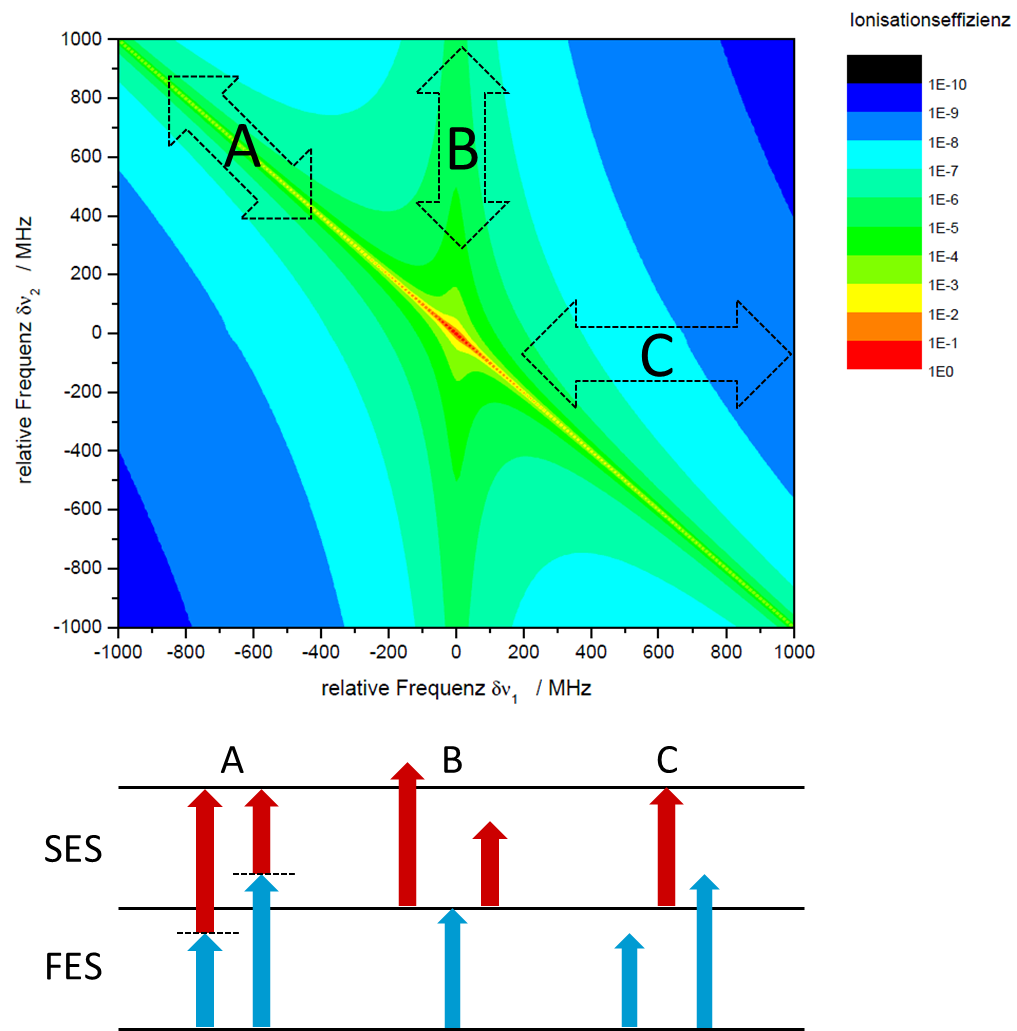
\includegraphics[width=15cm]{gfx/2d-laserscan_theorie_schumann.png}
	\caption{Dopplerfreie
	Ionisationseffizienz in Abhängigkeit
	der Verstimmungen der beiden ersten
	Anregungsschritte mit den Strukturen
	der Einphoton-Resonanz (B), (C) und
	Zweiphotonen-Resonanz (A),
	Erklärung im Text}\label{fig:2D-laserscan_theorie_schumann}
\end{figure}
Wie die interessanten Strukturen zeigen, ergibt sich kein zweidimensionales
Voigtprofil, wie man es naiverweise annehmen könnte. Die diagonale Struktur A
resultiert aus der \textit{Zweiphotonen-Resonanz}. Dabei ist die Summenfrequenz
der ersten beiden Anregungsschritte gleich der Übergangsfrequenz vom
Grundzustand zum zweiten angeregten Niveau. Auch bei relativ großer Verstimmung
zum Zwischenniveau erhält man noch signifikante Zählraten. Die Struktur B
zeigt die \textit{Einphotonen-Resonanz} bei resonantem ersten Übergang. Auch
hier ergeben sich signifikante Zählraten bei großer Verstimmung des zweiten Schrittes, aber
wesentlich weniger als bei der Zweiphotonen-Resonanz. Hält man im Gegensatz dazu
den zweiten Schritt resonant fest und verstimmt den ersten Schritt, fällt die
Ionisatzionseffizient sehr schnell ab (C). Dies ist leicht einzusehen, denn es
ist bei mehrfach resonanter Anregung wesentlich effizienter, wenn die starke
Populationsabnahme durch nicht-Resonanz erst in höheren Niveaus eintritt als
schon in den unteren Niveaus.

\subsection{Ionisation}\label{subsec:ionisation}
Um die Atome letzendlich nach dem letzten Anregungsschritt zu ionisieren, muss
ein Niveau besetzt werden, das oberhalb des Ionisationspotentials liegt. Die
kann auf Grund drei verschiedener Prozesse geschehen: \textit{Feldionisation},
\textit{nicht-resonante Photoionisation} und \textit{Autoionisation}. Da die
ersten beiden Prozesse in diesem Projekt keine keine Anwendung finden bzw.
keinen merkenswerten Beitrag haben, seien diese nur am Rande erwähnt und es soll
näher auf die Autoionisation eingegangen werden.

\subsubsection{Feldionisation}\label{subsubsec:feldionisation}
Durch Anlegen eines elektrischen Feldes in der Wechselwirkungsregion mit des
Lasern kann das Ionisationspotential herabgesenkt werden, wodurch gebundene
Zustände oberhalb des Ionisationspotentials liegen können und somit durch
resonante Anregung in diese Zustände eine Ionisation möglich ist. Da allerdings
hierfür sehr starke Felder nötig sind, kommt es ungünstigerweise zu
\textit{AC-Stark-Shifts} insbesondere in den Niveaus der unteren Schritte.

\subsubsection{nicht-resonante
Photoionisation}\label{subsubsec:nicht-resonante_photoionisation}
Neben resonanten Übergängen sind auch nicht-resonante Anregungen in das
Kontinuum möglich. Vorraussetzung hierfür ist, dass die gesamte Photonenenergie
aller Anregungsschritte inklusive der Photonenenergie des ionisierenden Schritts
größer sein muss als die Energie des Ionisationspotentials
($\hbar\omega_1+\hbar\omega_2+\hbar\omega_3>\E_{IP}$). Da jedoch der
Wirkungsquerschnitt für solch einen Prozess gegenüber der anderen Prozesse
sehr unterdrückt ist, wird hierfür ein leistungsstarker Laser
benötigt, was wiederum mit erheblichen Kosten verbunden ist.

\subsubsection{Autoionisation}\label{subsubsec:autoionisation}
Bei der in diesem Projekt verwendeten Autoionisation sind Zustände nötig, die
oberhalb des Ionisationspotentials liegen. Bei komplexen Atomen wie das hier
verwendete Uran kommt es häufig vor, dass bestimmte Anregungsschritte durch die
Anregung zweier Elektronen charakterisiert sind. Obwohl diese Zustände
gebunden sind, kann ihre Gesamtenergie höher als das Ionisationspotential
liegen. Weiterhin gibt es starke Überlappe der Elektronen-Wellenfunktionen, was einen Energieübertrag zwischen zwei Elektronen begünstigt und so zu sehr schnellen
Zerfällen in ein Elektron und ein Ion führt. Die Lebensdauer solcher Zustände
kann bis zu 3-4 Größenordnungen kleiner sein als die der Zustände unterhalb des
Ionisationspotentials, wobei die spektrale Breite gemäß der
Unschärferelation entsprechend größer ist. Der Vorteil gegenüber den anderen
Prozessen ist die Möglichkeit, Atome ohne störende Einflüsse (Stark-Shifts)
resonant zu ionisieren, wobei für den ionisierenden Schritt nur moderate cw\footnote{cw:
"`continuous wave"', zu deutsch: "`kontinuierliche Welle"', Bezeichnung für Dauerstrichlaser}-Laserleistungen von
wenigen $100\,$mW nötig sind und gleichzeitig vergleichbar hohe
Wirkungsquerschnitte erzielt werden. Die autoionisierenden Übergänge sind
allerdings ununterscheidbar von den nicht-resonanten Prozessen, wodurch
beide Prozesse miteinander interferieren. Dazu betrachtet man als Endzustand
eine Linearkombination aus einem diskreten Niveau und dem Kontinuum:
\begin{equation}\label{eq:uebergang_diskret_kontinuum}
	\ket{E}=a\ket{\phi}+\int b_\epsilon\ket{\epsilon}\dd\epsilon\,.
\end{equation}
Nach einem zeitunabhängigen störungstheoretischen Ansatz
\begin{equation}\label{eq:uebergang_diskret_kontinuum_hamilton}
	\OPH=\OPH_0+V
\end{equation}
mit $\OPH_0$ als ungestörten, in der Basis
$\left(\ket{\phi}\text{,}\,\ket{\epsilon}\right)$ diagonalisierten
Hamiltonoperator und der Störung $V$ findet man nach längerer Rechnung,
welche in \cite{fano:1961:PhysRev.124.1866} ausgeführt ist, den
Wirkungsquerschnitt
\begin{equation}\label{eq:fano-profil}
	\sigma(q,\Gamma,E_0,\epsilon)=\frac{\left(\nicefrac{q\Gamma}{2}+\epsilon-E_0\right)^2}{\left(\epsilon-E_0\right)^2+\left(\nicefrac{\Gamma}{2}\right)^2}
\end{equation}
der autoionisierenden Resonanz. Dabei sind $q$ der Formparameter, $\Gamma$ die
Linienbreite und $E_0$ die Energielage der Resonanz. In \ref{fig:fano} ist der
Wirkungsquerschnitt als sog. \textit{Fano-Profil} noch einmal grafisch
dargestellt.
\begin{figure}
	\centering
	% GNUPLOT: LaTeX picture with Postscript
\begingroup
  \makeatletter
  \providecommand\color[2][]{%
    \GenericError{(gnuplot) \space\space\space\@spaces}{%
      Package color not loaded in conjunction with
      terminal option `colourtext'%
    }{See the gnuplot documentation for explanation.%
    }{Either use 'blacktext' in gnuplot or load the package
      color.sty in LaTeX.}%
    \renewcommand\color[2][]{}%
  }%
  \providecommand\includegraphics[2][]{%
    \GenericError{(gnuplot) \space\space\space\@spaces}{%
      Package graphicx or graphics not loaded%
    }{See the gnuplot documentation for explanation.%
    }{The gnuplot epslatex terminal needs graphicx.sty or graphics.sty.}%
    \renewcommand\includegraphics[2][]{}%
  }%
  \providecommand\rotatebox[2]{#2}%
  \@ifundefined{ifGPcolor}{%
    \newif\ifGPcolor
    \GPcolortrue
  }{}%
  \@ifundefined{ifGPblacktext}{%
    \newif\ifGPblacktext
    \GPblacktexttrue
  }{}%
  % define a \g@addto@macro without @ in the name:
  \let\gplgaddtomacro\g@addto@macro
  % define empty templates for all commands taking text:
  \gdef\gplbacktext{}%
  \gdef\gplfronttext{}%
  \makeatother
  \ifGPblacktext
    % no textcolor at all
    \def\colorrgb#1{}%
    \def\colorgray#1{}%
  \else
    % gray or color?
    \ifGPcolor
      \def\colorrgb#1{\color[rgb]{#1}}%
      \def\colorgray#1{\color[gray]{#1}}%
      \expandafter\def\csname LTw\endcsname{\color{white}}%
      \expandafter\def\csname LTb\endcsname{\color{black}}%
      \expandafter\def\csname LTa\endcsname{\color{black}}%
      \expandafter\def\csname LT0\endcsname{\color[rgb]{1,0,0}}%
      \expandafter\def\csname LT1\endcsname{\color[rgb]{0,1,0}}%
      \expandafter\def\csname LT2\endcsname{\color[rgb]{0,0,1}}%
      \expandafter\def\csname LT3\endcsname{\color[rgb]{1,0,1}}%
      \expandafter\def\csname LT4\endcsname{\color[rgb]{0,1,1}}%
      \expandafter\def\csname LT5\endcsname{\color[rgb]{1,1,0}}%
      \expandafter\def\csname LT6\endcsname{\color[rgb]{0,0,0}}%
      \expandafter\def\csname LT7\endcsname{\color[rgb]{1,0.3,0}}%
      \expandafter\def\csname LT8\endcsname{\color[rgb]{0.5,0.5,0.5}}%
    \else
      % gray
      \def\colorrgb#1{\color{black}}%
      \def\colorgray#1{\color[gray]{#1}}%
      \expandafter\def\csname LTw\endcsname{\color{white}}%
      \expandafter\def\csname LTb\endcsname{\color{black}}%
      \expandafter\def\csname LTa\endcsname{\color{black}}%
      \expandafter\def\csname LT0\endcsname{\color{black}}%
      \expandafter\def\csname LT1\endcsname{\color{black}}%
      \expandafter\def\csname LT2\endcsname{\color{black}}%
      \expandafter\def\csname LT3\endcsname{\color{black}}%
      \expandafter\def\csname LT4\endcsname{\color{black}}%
      \expandafter\def\csname LT5\endcsname{\color{black}}%
      \expandafter\def\csname LT6\endcsname{\color{black}}%
      \expandafter\def\csname LT7\endcsname{\color{black}}%
      \expandafter\def\csname LT8\endcsname{\color{black}}%
    \fi
  \fi
  \setlength{\unitlength}{0.0500bp}%
  \begin{picture}(7200.00,5040.00)%
    \gplgaddtomacro\gplbacktext{%
      \csname LTb\endcsname%
      \put(740,859){\makebox(0,0)[r]{\strut{} 0}}%
      \put(740,1297){\makebox(0,0)[r]{\strut{} 2}}%
      \put(740,1734){\makebox(0,0)[r]{\strut{} 4}}%
      \put(740,2172){\makebox(0,0)[r]{\strut{} 6}}%
      \put(740,2610){\makebox(0,0)[r]{\strut{} 8}}%
      \put(740,3048){\makebox(0,0)[r]{\strut{} 10}}%
      \put(740,3486){\makebox(0,0)[r]{\strut{} 12}}%
      \put(740,3923){\makebox(0,0)[r]{\strut{} 14}}%
      \put(740,4361){\makebox(0,0)[r]{\strut{} 16}}%
      \put(740,4799){\makebox(0,0)[r]{\strut{} 18}}%
      \put(1458,440){\makebox(0,0){\strut{}-4}}%
      \put(2654,440){\makebox(0,0){\strut{}-2}}%
      \put(3849,440){\makebox(0,0){\strut{} 0}}%
      \put(5045,440){\makebox(0,0){\strut{} 2}}%
      \put(6241,440){\makebox(0,0){\strut{} 4}}%
      \put(160,2719){\rotatebox{-270}{\makebox(0,0){\strut{}Wirkungsquerschnitt $\sigma$}}}%
      \put(3849,140){\makebox(0,0){\strut{}Energie $\epsilon$}}%
    }%
    \gplgaddtomacro\gplfronttext{%
      \csname LTb\endcsname%
      \put(1340,4636){\makebox(0,0)[r]{\strut{}q=0}}%
      \csname LTb\endcsname%
      \put(1340,4436){\makebox(0,0)[r]{\strut{}q=1}}%
      \csname LTb\endcsname%
      \put(1340,4236){\makebox(0,0)[r]{\strut{}q=2}}%
      \csname LTb\endcsname%
      \put(1340,4036){\makebox(0,0)[r]{\strut{}q=3}}%
      \csname LTb\endcsname%
      \put(1340,3836){\makebox(0,0)[r]{\strut{}q=4}}%
    }%
    \gplbacktext
    \put(0,0){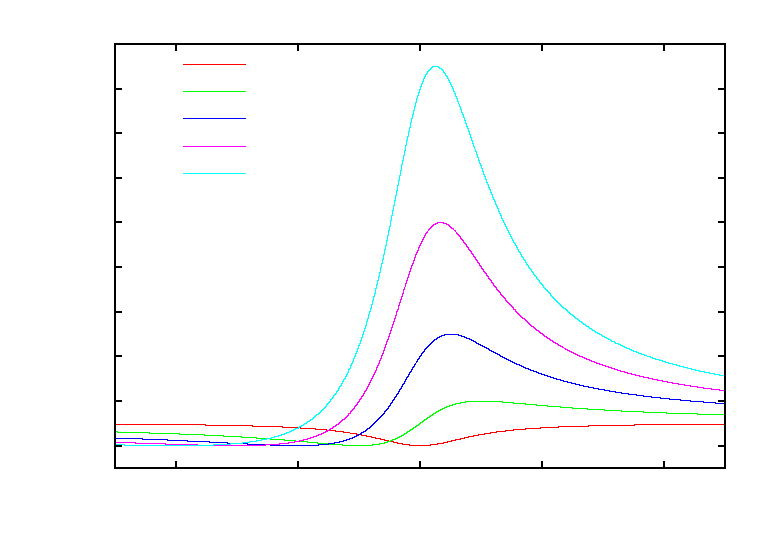
\includegraphics{fano}}%
    \gplfronttext
  \end{picture}%
\endgroup

	\caption{Fano-Profil gemäß Gl. \eqref{eq:fano-profil} mit
	$\Gamma=2$, $E_0=0$ und verschiedenen $q$}\label{fig:fano}
\end{figure}
Man erkennt, dass es sowohl konstruktive (Maximum) als auch destruktive
(Minimum) Interferenzen zwischen den Übergängen in das Kontinuum und Übergänge
in einen diskreten Zustand gibt. Für $q=0$ findet man bei $\epsilon=0$ ein
Minimum, die sog. \textit{Window-Resonanz}. Für große $q$ ist die Überhöhung der
Autoionisation gegenüber der nicht-resonanten Photoionisation näherungsweise
quadratisch mit $q$ und $\sigma$ nähert sich einem Lorentzprofil.\par
Komplizierter wird die Beschreibung, wenn man mit einbezieht, dass verschiedene
Resonanzen und auch Kontinua miteinander interfereieren. Dazu wird allgemein ein
Streuprozess betrachtet, bei dem das vor der Streuung gebundene Elektron am
Ion streut und für $t\to\infty$ sich ein freies Ion-Elektron-System ergibt. Dies
lässt sich gut mit der \textit{K-Matrix Theorie} beschreiben. Nach
\cite{connerade:1998:highly_excited_atoms} ergibt sich dann für den
Wirkungsquerschnitt
\begin{equation}\label{eq:k-matrix_wirkungsquerschnitt}
	\sigma\left(q_{1..n},\Gamma_{1..n},E_{1..n},E\right)=\abs{\tilde{D}}^2\frac{\left(1+\sum\limits_{k=1}^n{\frac{\nicefrac{\Gamma_k}{2}}{\left(E_k-E\right)}q_k}\right)^2}{1+\left(\sum\limits_{k=1}^n{\frac{\nicefrac{\Gamma_k}{2}}{\left(E_k-E\right)}}\right)^2}\,.
\end{equation}
Für zwei interferierende Resonanzen wurde der Wirkungsquerschnitt in Fig.
\ref{fig:k-matrix_wirkungsquerschnitt} aufgetragen.
\begin{figure}
	\centering
	% GNUPLOT: LaTeX picture with Postscript
\begingroup
  \makeatletter
  \providecommand\color[2][]{%
    \GenericError{(gnuplot) \space\space\space\@spaces}{%
      Package color not loaded in conjunction with
      terminal option `colourtext'%
    }{See the gnuplot documentation for explanation.%
    }{Either use 'blacktext' in gnuplot or load the package
      color.sty in LaTeX.}%
    \renewcommand\color[2][]{}%
  }%
  \providecommand\includegraphics[2][]{%
    \GenericError{(gnuplot) \space\space\space\@spaces}{%
      Package graphicx or graphics not loaded%
    }{See the gnuplot documentation for explanation.%
    }{The gnuplot epslatex terminal needs graphicx.sty or graphics.sty.}%
    \renewcommand\includegraphics[2][]{}%
  }%
  \providecommand\rotatebox[2]{#2}%
  \@ifundefined{ifGPcolor}{%
    \newif\ifGPcolor
    \GPcolortrue
  }{}%
  \@ifundefined{ifGPblacktext}{%
    \newif\ifGPblacktext
    \GPblacktexttrue
  }{}%
  % define a \g@addto@macro without @ in the name:
  \let\gplgaddtomacro\g@addto@macro
  % define empty templates for all commands taking text:
  \gdef\gplbacktext{}%
  \gdef\gplfronttext{}%
  \makeatother
  \ifGPblacktext
    % no textcolor at all
    \def\colorrgb#1{}%
    \def\colorgray#1{}%
  \else
    % gray or color?
    \ifGPcolor
      \def\colorrgb#1{\color[rgb]{#1}}%
      \def\colorgray#1{\color[gray]{#1}}%
      \expandafter\def\csname LTw\endcsname{\color{white}}%
      \expandafter\def\csname LTb\endcsname{\color{black}}%
      \expandafter\def\csname LTa\endcsname{\color{black}}%
      \expandafter\def\csname LT0\endcsname{\color[rgb]{1,0,0}}%
      \expandafter\def\csname LT1\endcsname{\color[rgb]{0,1,0}}%
      \expandafter\def\csname LT2\endcsname{\color[rgb]{0,0,1}}%
      \expandafter\def\csname LT3\endcsname{\color[rgb]{1,0,1}}%
      \expandafter\def\csname LT4\endcsname{\color[rgb]{0,1,1}}%
      \expandafter\def\csname LT5\endcsname{\color[rgb]{1,1,0}}%
      \expandafter\def\csname LT6\endcsname{\color[rgb]{0,0,0}}%
      \expandafter\def\csname LT7\endcsname{\color[rgb]{1,0.3,0}}%
      \expandafter\def\csname LT8\endcsname{\color[rgb]{0.5,0.5,0.5}}%
    \else
      % gray
      \def\colorrgb#1{\color{black}}%
      \def\colorgray#1{\color[gray]{#1}}%
      \expandafter\def\csname LTw\endcsname{\color{white}}%
      \expandafter\def\csname LTb\endcsname{\color{black}}%
      \expandafter\def\csname LTa\endcsname{\color{black}}%
      \expandafter\def\csname LT0\endcsname{\color{black}}%
      \expandafter\def\csname LT1\endcsname{\color{black}}%
      \expandafter\def\csname LT2\endcsname{\color{black}}%
      \expandafter\def\csname LT3\endcsname{\color{black}}%
      \expandafter\def\csname LT4\endcsname{\color{black}}%
      \expandafter\def\csname LT5\endcsname{\color{black}}%
      \expandafter\def\csname LT6\endcsname{\color{black}}%
      \expandafter\def\csname LT7\endcsname{\color{black}}%
      \expandafter\def\csname LT8\endcsname{\color{black}}%
    \fi
  \fi
  \setlength{\unitlength}{0.0500bp}%
  \begin{picture}(7200.00,5040.00)%
    \gplgaddtomacro\gplbacktext{%
      \csname LTb\endcsname%
      \put(1342,704){\makebox(0,0)[r]{\strut{} 1000}}%
      \put(1342,1937){\makebox(0,0)[r]{\strut{} 10000}}%
      \put(1342,3171){\makebox(0,0)[r]{\strut{} 100000}}%
      \put(1342,4404){\makebox(0,0)[r]{\strut{} 1e+006}}%
      \put(1474,484){\makebox(0,0){\strut{}-100}}%
      \put(2235,484){\makebox(0,0){\strut{} 0}}%
      \put(2997,484){\makebox(0,0){\strut{} 100}}%
      \put(3758,484){\makebox(0,0){\strut{} 200}}%
      \put(4519,484){\makebox(0,0){\strut{} 300}}%
      \put(5280,484){\makebox(0,0){\strut{} 400}}%
      \put(6042,484){\makebox(0,0){\strut{} 500}}%
      \put(6803,484){\makebox(0,0){\strut{} 600}}%
      \put(176,2739){\rotatebox{-270}{\makebox(0,0){\strut{}$\sigma$}}}%
      \put(4138,154){\makebox(0,0){\strut{}E}}%
    }%
    \gplgaddtomacro\gplfronttext{%
      \csname LTb\endcsname%
      \put(2794,4581){\makebox(0,0)[r]{\strut{}$q_1=50$}}%
      \csname LTb\endcsname%
      \put(2794,4318){\makebox(0,0)[r]{\strut{}$q_1=100$}}%
      \csname LTb\endcsname%
      \put(2794,4055){\makebox(0,0)[r]{\strut{}$q_1=200$}}%
      \csname LTb\endcsname%
      \put(2794,3792){\makebox(0,0)[r]{\strut{}$q_1=300$}}%
      \csname LTb\endcsname%
      \put(2794,3529){\makebox(0,0)[r]{\strut{}$q_1=400$}}%
    }%
    \gplbacktext
    \put(0,0){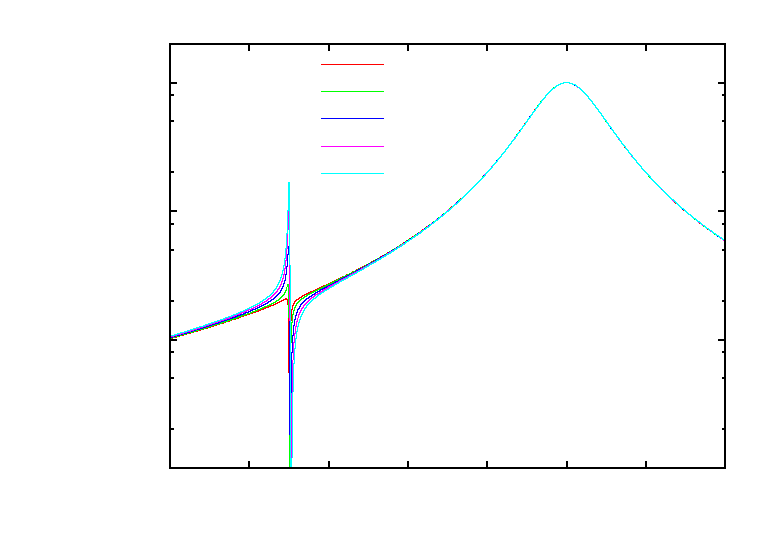
\includegraphics{k-matrix_wirkungsquerschnitt}}%
    \gplfronttext
  \end{picture}%
\endgroup

	\caption{Wirkungsquerschnitt gemäß Gl. \eqref{eq:k-matrix_wirkungsquerschnitt}
	mit $q_2=1000$, $E1=50$, $E2=400$, $\Gamma_1=2$, $\Gamma_2=2$ und
	verschiedenen $q_1$}\label{fig:k-matrix_wirkungsquerschnitt}
\end{figure}
Danach haben schmale Resonanzen ein asymetrisches Fano-Profil, wenn sie durch
eine benachbarte breite Resonanz gestört werden. Auch zu erkennen ist, dass
Resonanzen mit relativ zu anderen Resonanzen kleinem $q$ wie Window-Resonanzen
erscheinen.

\subsection{Uran}\label{subsec:uran}

\subsection{Isotopieverschiebung}\label{subsec:isotopieverschiebung}
Aufgrund der verschiedenen Kerne verschiedener Isotope kommt es zu
Energieniveauverschiebungen:
\begin{equation}\label{eq:isotopieshift}
	\delta\nu_{IV}=\delta\nu_{ME}+\delta\nu_{FE}\,.
\end{equation}
Diese Verschiebungen liegen zwischen einigen $100\,$MHz und einigen GHz. In
Relation zur Gesamtenergie eines Niveaus, welche bei einigen $100\,$THz liegt,
sind diese Verschiebungen zwar sehr klein, spielen aber z.B. bei
Isotopenverhältnisbestimmungen eine große Rolle. Gerade mit schmalbandigen
cw-Lasern lassen sich dadurch Isotope selektiv anregen. Die Verschiebung ist zum
einen durch die Massenänderung und zum anderen durch die veränderte Ladungsverteilung des Kerns zu begründen (Masseneffekt $\delta\nu_{ME}$ und Feldeffekt $\delta\nu_{FE}$ in \eqref{eq:isotopieshift}). Der Masseneffekt
\begin{equation}\label{eq:masseneffekt}
	\delta\nu_{ME}=K_{ME}\frac{m_{A'}-m_A}{m_{A'}m_A}
\end{equation}
ist von den beiden Massen $m_{A'}$ und $m_A$ der Isotope und von der
Masseneffektkonstante $K_{ME}=K_{NME}+K_{SME}$ abhängig. Die
Masseneffektkonstante wiederum besteht aus dem normalen Masseneffekt
\begin{equation}\label{eq:normaler_masseneffekt}
	\delta\nu_{NME}=m_e\nu_A\frac{m_A}{m_A+m_e}\,,
\end{equation}
der aus der veränderten reduzierten Masse, die sich in einem
Ein-Elektronen-System ergeben würde, resultiert und dem speziefischen
Masseneffekt $K_{SME}$, der aus der Änderung der Korrelation aller
Elektronenimpulse folgt und bestenfalls nur numerisch abgeschätzt werden
kann. \par Da die Ortsanteile der Wellenfunktionen der Elektronen immer mit dem Ort des
Kerns überlappen, kommt es bei Veränderung der Kernladungsdichteverteilung auch
zu einer Energieniveauverschiebung:
\begin{equation}\label{eq:normaler_masseneffekt}
	\delta\nu_{FE}=K_{FE}\delta\mean{r^2}\,.
\end{equation}
Mit der Annahme, dass die Wellenfunktionen der Elektronen am Ort des Kerns
nicht stark variieren und in jedem Isotop die gleiche sphärische Symmetrie
vorliegt, kann die Änderung der Kernladungsdichteverteilung nach geraden
Potenzen entwickelt werden. In Gl. \eqref{eq:normaler_masseneffekt} wurde
die quadratische (niedrigste) Ordnung dieser Entwicklung eingesetzt.\par
In der Anwendung unterscheidet man zwischen dem \textit{level-isotop-shift}
(LIS) und dem \textit{transition-isotop-shift} (TIS). Bei ersterem betrachtet
man die Energieverschiebung zwischen den Isotopen in Relation zum jeweiligen
Grundzustandsniveau:
\begin{equation}\label{eq:LIS}
	\delta\nu_{IV}^{LIS}(E)=\nu_{A_1}^{GZ_1\leftrightarrow
	E}-\nu_{A_2}^{GZ_2\leftrightarrow E}\,.
\end{equation}
Der TIS ist durch die Verschiebung des Abstands zweier Energieniveaus definiert:
\begin{equation}\label{eq:TIS}
	\delta\nu_{IV}^{TIS}(E',E)=\nu_{A_1}^{E'\leftrightarrow
	E}-\nu_{A_2}^{E'\leftrightarrow E}\,.
\end{equation}
Dies ist die in der Praxis sinnvollere Definition, da hier die Verschiebung
angibt, wie weit das Laserlicht beim Isotopenwechsel verstimmt werden muss, um
den gleichen Übergang zum Anregen des Isotops zu verwenden. LIS und TIS sind
über
\begin{equation}\label{eq:TIS_LIS_verknuepfung}
	\delta\nu_{IV}^{TIS}(E',E)=\delta\nu_{IV}^{LIS}(E)-\delta\nu_{IV}^{LIS}(E')
\end{equation}
miteinander verknüpft.

\section{Diodenlaser in der RIS}\label{sec:diodenlaser}